\chapter{Cluster-Based Channel Estimation}
\label{c:cluster_ce}

\begin{figure}[b!]
 \centering
 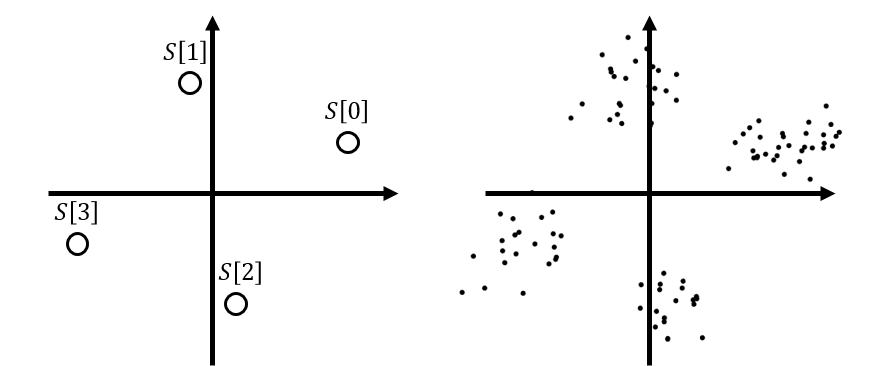
\includegraphics[width=15cm]{fig/rx_sig_m1_p2.bmp}
 \caption{Superimposed levels and the corresponding received signals in the case of $m=1$ and $U=2$.}
 \label{fig:rx_sig_m1_p2}
\end{figure}

In the thesis \cite{yt19}, the cluster-based channel estimation technique was proposed for efficient transmission. It used different clustering algorithms to analyze the mean square error (MSE) performance. However, it still couldn't achieve to  Cramer-Rao lower bound (CRLB) when $U$ was higher than two, and the proposed methods\cite{yt19} for deriving channel coefficients was a particular case that was only suitable for $U=2$ or $U=3$.  Hence, we proposed a general algorithm for clustering received signals and deriving the channel coefficient for any user and modulation.

\paragraph{Introduction for Cluster-based Channel Estimation}

When multiple users transmit through independent fading channels, the signals can be further separated by using different channel coefficients without requiring user-specific resources. The requirement for applying multi-level detection in the GDMA system is to accurately recover the channel coefficients at the receiver to construct all possible superimposed signal levels. Due to the presence of channel noise, the received signal in the block where the channel remains unchanged has a two-dimensional Gaussian distribution with mean $S[l]$ where $l \in \{0 \ ,1 \ , \cdots \ , 2^{mU} \}$ according to the messages of $U$ users. If we can classify the received symbols into a $2 ^ {mU} $ group in some way, where the symbols corresponding to the same level are grouped, the estimated value of the level can be obtained by the average value of the symbols in each group. In this section, we assume that he fading coefficients are constant across a block of $N_t$ consecutive symbols.  An example of the receive signals with $N_t$= 100 in the case of $m=1$ and $U=2$ is shown in Fig.\ref{fig:rx_sig_m1_p2}. Therefore, we use clustering algorithm to classify the received signals and blindly estimate the channel coefficients of $U$ users. Clustering is an unsupervised learning technique, which involves grouping training samples from different groups with different characteristics. Note that the clustering technique in the proposed scheme takes the signal with message as the input training sample, and since the estimation does not require additional pilot signals, it can achieve high frequency spectral efficiency and inevitable ambiguity in estimation.

%==================================================

\section{Review of Clustering Algorithm}

 Clustering is an unsupervised learning technique and the task of grouping a set of objects that called a cluster. In this section, we review the clustering algorithm survey from the thesis \cite{yt19}.

\subsection{K-Means Algorithm}
\label{s:clustering}

One of the most popular clustering techniques is the k-mean algorithm\cite {lloyd82}, which aims to minimize the sum of the square distance between each sample and its closest centroid. In the k-means problem, it is desirable to choose a set of centroids $S$ such that the following function can be minimized.

\begin{equation}
 \phi = \sum_{x \in X} \underset{s \in S}{\text{min}} \parallel x-s \parallel^2,
\end{equation}
where $X$ is the set of training vectors, and $\phi$ is the corresponding distortion. Therefore, K-means algorithm classifies samples by iteratively pairing each sample with the closest centroid, and then updating the centroid from the newly derived group.

For channel estimation in the GDMA system, all the levels should be distinguished. The number of groups to be classified is $2^{mU}$ in the clustering. The steps of the k-means algorithm are organized as follows.
\begin{enumerate}[leftmargin=\leftmargin+\widthof{Prefix}]
\item[Step 1)] Randomly pick the initial centroids from the symbols in the received sequence.
\item[Step 2)] Classify the received symbols into $2^{mU}$ groups by applying the nearest-neighbor rule with respect to the current centroids.
\item[Step 3)] Recompute the centroids by averaging the symbols in each group.
\item[Step 4)] Return to Step 2 until the centroids no longer change.
\end{enumerate}
The required number of iterations for clustering algorithms cannot be predicted ahead of time. In addition, the random seeding in the initial step of k-means may yield different grouping results in different runs of the algorithm.

In the k-means algorithm, the most crucial task is selecting acceptable initial centroids in the correct solution's neighborhood since it can only find a local minimum. Several clustering algorithms was proposed to select acceptable initial centroids such as LBG algorithm, k-mean++ algorithm, modified k-means++ algorithm.

%--------------------------------------------------

\subsection{The LBG Algorithm}

The Linde–Buzo–Gray (LBG) algorithm \cite{lbg80}, sometimes referred to as generalized Lloyd algorithm (GLA), is a technique to design vector quantizer and a so-called "splitting" method is employed to select the initial centroids for the following k-means clustering. The steps of LBG algorithm are organized as follows.
\begin{enumerate}[leftmargin=\leftmargin+\widthof{Prefix}]
\item[Step 1)] Split the origin into two close points $\epsilon$ and $-\epsilon$ and hence the set of initial centroids $S=\{\epsilon,-\epsilon\}$ with size $M=2$ is obtained.
\item[Step 2)] Classify the received symbols into $M$ groups, based on the current centroids $S$, by applying the nearest-neighbor rule and compute the centroid $\rho_i$ of each group with $i \in \{1, 2, ..., M\}$.
\item[Step 3)] Split $\rho_i$ into two close points $q_{2i-1}=\rho_i+\epsilon$ and $q_{2i}=\rho_i-\epsilon$ with $i \in \{1, 2, ..., M\}$ and the set of new centroids $S=\{q_i| i=1, 2, ...,2M\}$ is obtained.
\item[Step 4)] Replace $M$ by $2M$ and return to Step 2 until $M=2^{mU}$.
\item[Step 5)] Proceed with the standard k-means clustering.
\end{enumerate}

\begin{figure}[t!]
 \centering
 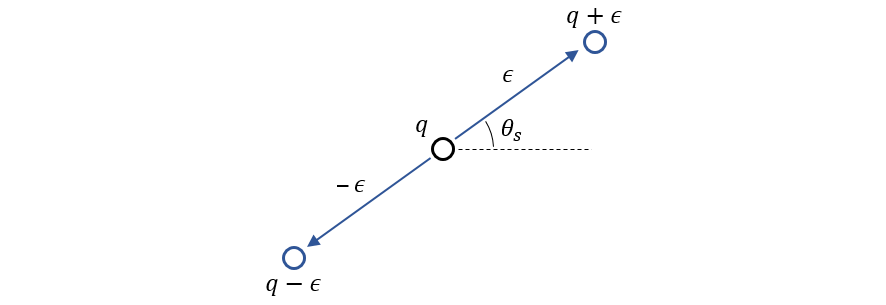
\includegraphics[width=15cm]{fig/lbg_splitting.png}
 \caption{Splitting from $q$ to get $q+\epsilon$ and $q-\epsilon$ with a perturbation vector $\epsilon$.}
 \label{fig:lbg_splitting}
\end{figure}

%--------------------------------------------------

\subsection{K-Means++ Algorithm}

The K-means + + algorithm is proposed in the \ {kmpp07} to select the initial centroid for the following K-means clustering, which can be regarded as a generalization of the standard k-means algorithm. The concept of K-means + + algorithm is to select the initial centroid as randomly as possible. Note that randomness is preserved in initialization, so K-means + + may not rely on the accuracy of training samples as LBG does. Let $D(r)$denote the distance from the received symbol $r$ to the closest centroid we have selected.

The steps of k-means++ algorithm are organized as follows.
\begin{enumerate}[leftmargin=\leftmargin+\widthof{Prefix}]
\item[Step 1)] Pick the first centroid $q_1$ uniformly at random from the symbols in received sequence and set $i=1$.
\item[Step 2)] Pick the next centroid $q_{i+1}$ from the remaining symbols with probability proportional to $D^2(r)$ and replace $i$ by $i+1$.
\item[Step 3)] Return to Step 2 until $i=2^{mU}$.
\item[Step 4)] Proceed with the standard k-means clustering.
\end{enumerate}


\subsection{Modified K-Means++ Algorithm}

The modified k-means++ algorithm was proposed in \cite{hsu2020uplink} to choose the initial centroids for the following k-means clustering, which can also be seen as a generalization of standard k-means algorithm. Compared to the k-means++ algorithm, it restricts the search space to a set $\Omega$ when selecting the next centroid $q_{i+1}$. This restriction might decrease the probability of selecting unsuitable initial centroids and still maintaining the randomness property for selecting centroids. Let $D(r)$ denote the distance from a received symbol $r$ to the closest centroid we have already chosen. The steps of the modified k-means++ algorithm are organized as follows.
\begin{enumerate}[leftmargin=\leftmargin+\widthof{Prefix}]
\item[Step 1)] Pick the first centroid $q_1$ uniformly at random from the symbols in received sequence and set $i=1$.
\item[Step 2)] Compute $D(r)$ which is the shortest distance between $r \in {\bf r}$ and any initial centroid in $\{q_1, ..., q_i\}$. Decide the set $\Omega$ that is comprised of $n/(2^{mU})$ symbols which have larger $D(r)$ values than those symbols in ${\bf r}\setminus\Omega$.   Select the next centroid $q_{i+1}$ from $\Omega$ according to a probability proportional to $D^2(r)$, and replace $i$ with $i+1$.
\item[Step 3)] Return to Step 2 until $i=2^{mU}$.
\item[Step 4)] Proceed with the standard k-means clustering.
\end{enumerate}

Compared above clustering algorithms, the modified k-means++ algorithm has the best performance in \cite{hsu2020uplink}, but it still cannot achieve the CRLB of MSE.  

%--------------------------------------------------

\subsection{Gaussian Mixture Model}

\begin{figure}[b!]
 \centering
 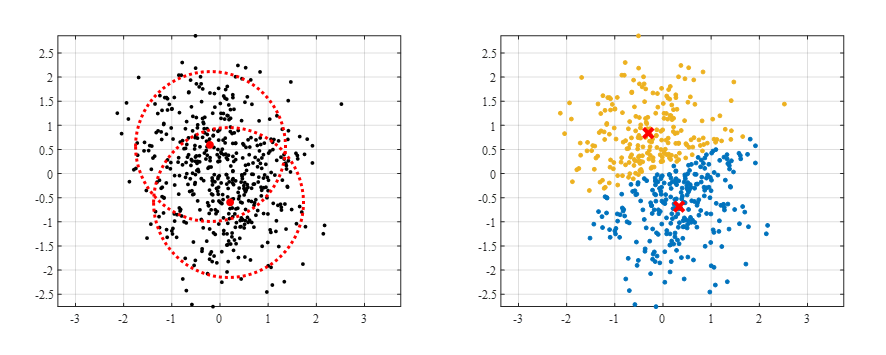
\includegraphics[width=15cm]{fig/hard_clustering.png}
 \caption{Grouping result of hard clustering by applying nearest neighbor rule.}
 \label{fig:hard_clustering}
\end{figure}

Clustering technology can be divided into two types: soft clustering and hard clustering. In hard clustering, each sample is accurately assigned to a group by applying the nearest neighbor rule. However, when samples from different sources are highly overlapped, it is difficult to tell which group the samples belong to in the overlap region.  In Fig.~\ref{fig:hard_clustering}, two sources produce samples with two-dimensional Gaussian distribution, and the mean values are represented as red dots. The Red Cross is the center of mass of the composition, and the color is shown in the figure Fig.~\ref{fig:hard_clustering}. The group classified by hard clustering in clustering.  Fig.~\ref{fig:hard_clustering} is the received symbol in BPSK modulation transmission of $U = 1 $user, and the SNR is relatively low. Therefore, the interference of channel noise makes it difficult to distinguish the two levels and reduces the accuracy of 
estimation.

Gaussian mixture model (GMM) is a method to realize soft clustering. It assumes that samples from different sources are Gaussian distributions with different parameters (mean and covariance). Therefore, the clustering problem is transformed into parameter optimization of Gaussian component in GMM. Expectation maximization (EM) algorithm \cite{em77} is usually used to find the parameters of Gaussian components in GMM. Since the channel noise is Gaussian distribution, the assumption of Gaussian component in GMM is suitable for the clustering of received symbols. In addition, as mentioned above, since the variance of each Gaussian component is equal to the variance of channel noise, and the probability of occurrence is equal, only the mean value of the component needs to be considered. For the signals received in GDMA system, the steps of EM cluster using GMM are as follows.

\begin{enumerate}[leftmargin=\leftmargin+\widthof{Prefix}]
\item[Step 1)] Initially set the occurrence probability $\text{Pr}(i)=2^{-mU}$ and the covariance matrix of Gaussian distribution is ${\bf \Sigma}_i = \sigma_w^2 {\bf I}_2$, where $\sigma_w^2$ is the variance of channel noise and ${\bf I}_2$ is a two-by-two unit matrix, for each component $i$ with $i \in \{1, 2, ..., 2^{mU}\}$.
\item[Step 2)] Proceed with k-means clustering and the resultant centroids are configured as the initial means of Gaussian components.
\item[Step 3)] Compute the soft assignment of each received symbol $r(n)$ by
\begin{equation}
 \text{Pr}(i|r(n)) = \frac{\mathcal{CN}(r(n)|\mu_i,{\bf \Sigma}_i)}{\sum_{j=1}^{2^{mU}}\mathcal{CN}(r(n)|\mu_j,{\bf \Sigma}_j)},
\end{equation}
where $i \in \{1,2,...,2^{mU}\}$ and $\mathcal{CN}$ denotes the PDF of complex Gaussian distribution.
\item[Step 4)] Derive the ML estimate of mean for component $i$ with
\begin{equation}
 \mu_i = \frac{1}{N_i} \sum_{n=1}^{N_t} r(n)\text{Pr}(i|r(n)),
\end{equation}
where $i \in \{1, 2, ..., 2^{mU}\}$ and $N_i=\sum_{n=1}^{N_t}\text{Pr}(i|r(n))$.
\item[Step 4)] Return to Step 3 until the means no longer change.
\end{enumerate}

The procedure of EM clustering is quite similar to that of the k-means algorithm, which needs the initialization of the parameters. Here we directly use the centroids derived from the k-means++ algorithm to be the initial means of Gaussian components in GMM, as stated in Step 2. After the EM clustering, the means of elements become the resultant centroids.

\section{Cluster-based Estimation Analysis and Design}

Cluster-based estimation can increase the efficiency of transmission, but it still has many problems. First, we analyzed how many samples are needed to achieve cluster reliability. Second, compared to \cite{yt19} only using the symmetric condition to judge whether it has correctly converged, we added more restrictions to increase algorithm security. Third, compared to the case where \cite{yt19} will plunge into fail loops to find correct convergence, we propose a method that can significantly reduce the number of iteration. Fourth, compared to the limitation \cite{yt19} of derivating channel coefficient, the algorithm we proposed can be applied in various cases.

\subsection{Clustering Sample Size Analysis}

The mean-square error (MSE) performances are simulated to evaluate the performance of cluster-based estimation applied to Rayleigh flat fading channels ,and the MSE is defined as

\begin{align}
\text{MSE}(h,\hat{h})=\frac{1}{2} | h,\hat{h} |^2  
\end{align}

where $h$ is the exact channel coefficient and $\hat{h}$ is the estimate of $h$. Note that the average energy of channel coefficient and transmitted signals are both normalized to one. The Cramer-Rao lower bound (CRLB), for the minimum variance unbiased (MVU) estimator using $N_t$ samples in the estimation, is also provided to evaluate the performance. Consider the observations when the signals are propagated through the channel with AWGN as
$r(n)=h+w(n),n=0,1,\cdots,N_t-1$.

\begin{figure}[b!]
 \centering
 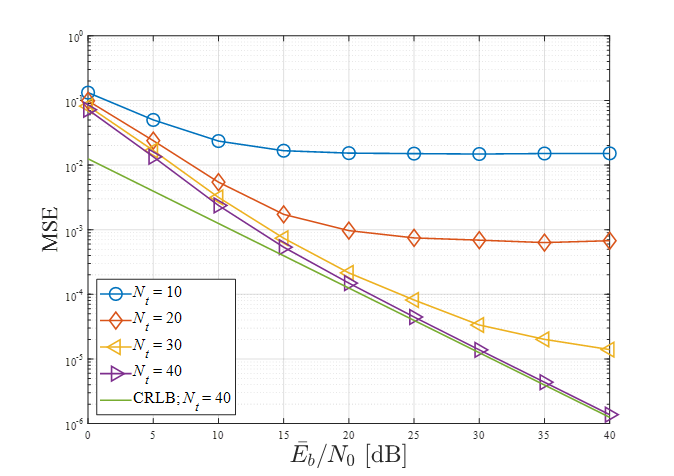
\includegraphics[width=15cm]{fig/sample_size_analysis1.png}
 \caption{MSE of estimated channel coefficient over AWGN channels.}
 \label{fig:sample_size_analysis1}
\end{figure}

,where $h$ is the parameter to be estimated and w(n) is AWGN with variance $\sigma_w^2$. The MVU estimator of h can be derived as 

\begin{align}
\hat{h} = \frac{1}{N_t} \sum_{n=0}^{N_t-1}r(n)  
\end{align}

and the variance of $\hat{h}$ is the CRLB written as

\begin{align}
\sigma^{2}_{h} = \frac{\sigma^{2}_{w}}{N_t}  
\end{align}

Assume that $U = 2$ and BPSK transmission, we changed the sample size arbitrarily. Observe the fig.\ref{fig:sample_size_analysis1} and find that the smaller the size, the earlier the error floor will occur. Because the number of samples is lack, some superimposed levels may not be generated and must lead to errors. We called it the worst case. In the following formula derivation, we derived the probability that the sample size will lead to the worst case.

Assume that $L=2^{mU}$ is the number of superimposed levels, $N_t$ is the number of clustering points and $A_i$ is the random variable that $i$-th superimposed level is empty where $i \in \{ 1, \ 2, \  \cdots, \  L \}$.

\begin{align}
& \text{Pr}{(A_i)} = {( \frac{L-1}{L} )}^{N_t} \nonumber \\
& \text{Pr}{(A_i \cap A_j)} = {( \frac{L-2}{L} )}^{N_t}, i \neq j  \ \nonumber \\
 & \quad \vdots \ \nonumber \\
& \text{Pr}{(A_i \cap A_j \cdots \cap A_r)} = {( \frac{1}{L} )}^{N_t}, i \neq j  \cdots \neq r \ 
\end{align}

\begin{align}
\text{Pr}{(\text{error})} &= \text{Pr}{(\text{at least one level is empty})} \ \nonumber \\
& = \text{Pr}{(A_i \cup A_j \cdots \cup A_r)} \ \nonumber \\
& = \text{C}^L_1 \ \text{Pr}{(A_i)} \ - \ \text{C}^L_2 \ \text{Pr}{(A_i \cup A_j)} \ + \ \text{C}^L_3 \ \text{Pr}{(A_i \cup A_j \cup A_j)} \ + \ \cdots  \nonumber \\
& + \ {(-1)}^{L-2} \ \text{C}^L_{L-1} \ \text{Pr}{(A_i \cup A_j \cup A_j \cdots)} \ \nonumber \\
& = \text{C}^L_1 \ {(\frac{L-1}{L})}^{N_t} \ - \ \text{C}^L_2 \ {(\frac{L-2}{L})}^{N_t} \ + \ \text{C}^L_3 \ {(\frac{L-1}{L})}^{N_t} \ + \ \cdots  + \ {(-1)}^{L-2} \ \text{C}^L_{L-1} \ {(\frac{1}{L})}^{N_t} \ 
\end{align}

\begin{figure}[H]
 \centering
 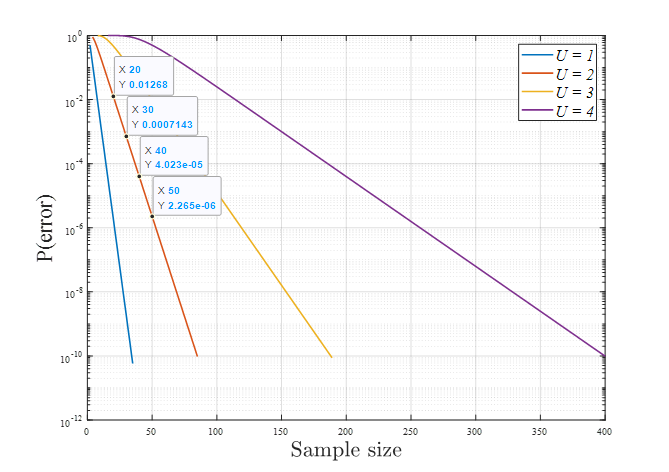
\includegraphics[width=15cm]{fig/sample_size_error_probability_analysis.png}
 \caption{The probability of worst case with BPSK transmission for different user $U$.}
 \label{fig:sample_size_error_rate}
\end{figure}

In Fig.\ref{fig:sample_size_error_rate}, derive the probability that superimposed levels is empty according to above equality. and list the following table.\ref{table:sample_size} that is probability with different clustering samples size. Fig.\ref{fig:sample_size_analysis} is the MSE of paired sample. Expect for $N_t=10$, sample size $N_t=20$ and $N_t=30$ both achieve the CRLB. 

\begin{table}[b!]
\caption{The probability that at least one superimposed level is empty for $L=4$.}
\begin{center}
 \begin{tabular}{ |c|c|c|c|c|c| }
 \hline
 Sample size & 10 & 20 & 30 & 40 & 50 \\
 \hline
 Pr\{error\}  & $0.2194$ & $0.01268$ & $7.143e^{-4}$ & $4.023e^{-5}$ & $2.265e^{-6}$ \\
 \hline
\end{tabular}
\end{center}
\label{table:sample_size}
\end{table}

\begin{figure}[t!]
 \centering
 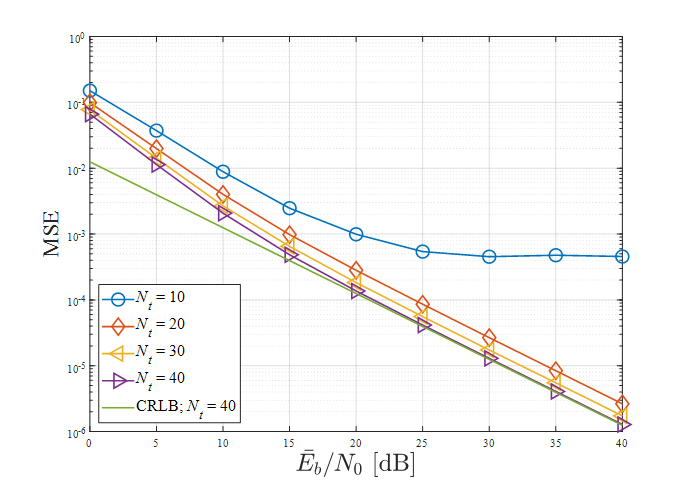
\includegraphics[width=15cm]{fig/sample_size_analysis.png}
 \caption{MSE of estimated channel coefficient with pair samples over AWGN channels.}
 \label{fig:sample_size_analysis}
\end{figure}


We can make up the problem according to the structure of modulation. Generate a sample with $\pi$ phase shift for BPSK transmission and create three copies of the received sample for QPSK transmission with $\frac{\pi}{2}, \ \pi ,\ \frac{3\pi}{2} $ phase shift respectively.

\subsection{Proposed Clustering Algorithm}

\begin{figure}[b!]
 \centering
 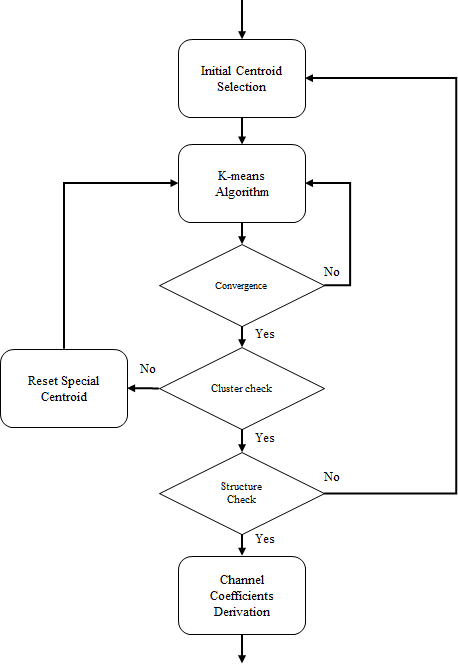
\includegraphics[width=10cm]{fig/flow_chart_proposed_clustering.png}
 \caption{The flow chart of proposed cluster-based channel estimation algorithm.}
 \label{fig:flow_chart_proposed_clustering}
\end{figure}

In the thesis \cite{yt19}, the main focus was on selecting good initial centroids, and a modified k-mean algorithm has also been proposed to make the initial centroid choosing better. In most of the clustering literature, it is mainly in the study of the initial centroids. Although the initial centroid selection is very important, it isn't easy to cluster correctly by completely modifying the initial selecting algorithm. We have come up with a different idea, not the study of initial centroids. The clustering algorithm in \cite{yt19} will re-execute if the symmetric condition is not met. The re-executed clusterings are independent of the previous one, resulting in inefficient or falling into a wrong loop. Hence, we came up with new ideas to make these re-executed clustering related to the last grouping and make them more efficient. Fig. \ref{fig:flow_chart_proposed_clustering} is the flow chart of proposed clustering algorithm. The cluster check is the algorithm to check whether convergence centroids are correct, roughly using the symmetric properties, group size, and group MSE. According to the cluster check, process the algorithm of resetting special centroids, which only reset the incorrect centroids. The structure check is the function to check centroids more accurately by using the superimposed level structure, and the channel coefficient derivation function is the novel algorithm different from \cite{yt19}.  The details of each flow block are described as the following subsection.


\subsubsection{Cluster Check}

In addition to selecting better initial centroids, we also change the algorithm after convergence. The fig.\ref{fig:cluster_check}-(a) is a cluster convergence case, but it does not conform to the superimposed levels symmetry condition. Thus, in the algorithm \cite{yt19}, the clustering algorithm would re-execute until the estimated centroids symmetry, but since each clustering algorithm is independent, it is possible to fall into a loop. Besides, even if it meets the symmetry condition, it could still be the wrong convergence.

Fig.\ref{fig:cluster_check}-(a), one case of convergence, it does not conform to the symmetric condition, but green centroids converge to the correct superimposed levels, where only red centroids do not. Hence, we can estimate whether those centroids converge correctly. Here, we use group MSE and group size to estimate centroids individually to check which centroid is reliable. 

Group MSE is the mean square error (MSE) of each cluster's centroid and its members. Under normal circumstances, group MSE should be similar to the noise variance. Therefore, if the group MSE is unusually large or small, this cluster is an error. Group MSE can be expressed as



\begin{align}
MSE_k = \sum^{N_{k}}_{i=0} \frac{{(r_{k,i} - C_k)}^2}{N_k}, \ k=1,2,\cdots,L
\end{align}

, where $N_k$ is the group size of $k$-th cluster, $C_k$ is the centroid of $k$-th cluster.


Group size is the number of members of each cluster. Under normal circumstances, the group size should be $\frac{N_t}{L}$ approximately and it can also be utensil to estimate. $N_k,k=1,2, \cdots, L$

We map group MSE or size into a reliability value for each centroid. If the value is smaller or larger than a threshold, label it a bad centroid. However, neither group MSE nor group size can not be entirely correct. We use them alternately until the estimated superimposed levels are the right structure.


\begin{figure}[t!]
 \centering
 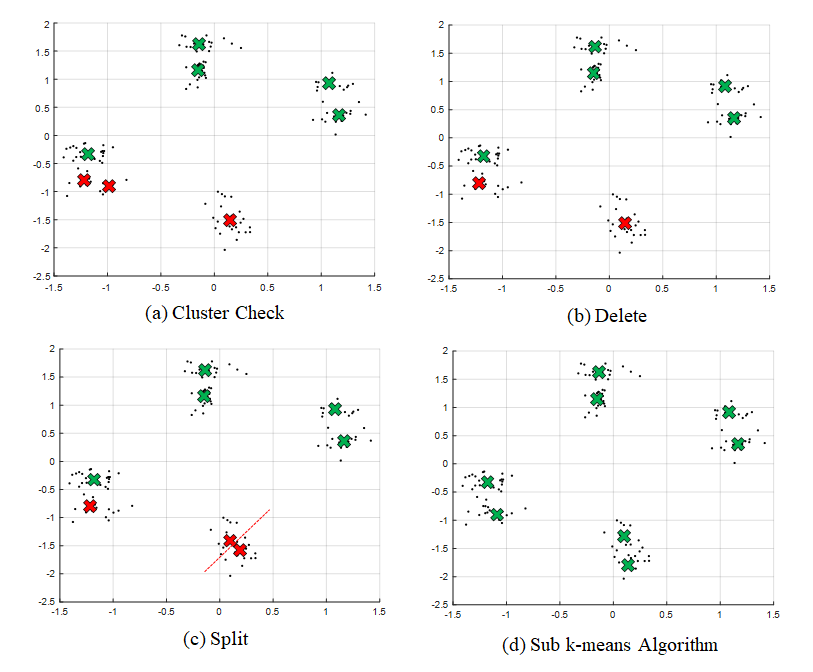
\includegraphics[width=14cm]{fig/cluster_check.png}
 \caption{An example of cluster check.}
 \label{fig:cluster_check}
\end{figure}

\begin{figure}[b!]
 \centering
 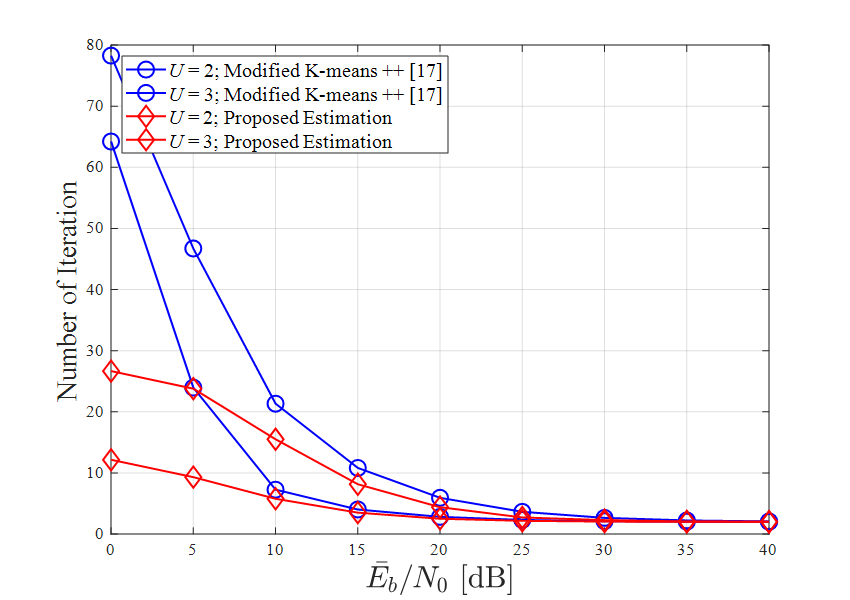
\includegraphics[width=14cm]{fig/channel_gain_iteration_128.png}
 \caption{The iteration number of estimated channel gain at $N_t=128$.}
 \label{fig:channel_gain_iteration_128}
\end{figure}


\subsubsection{Reset Special Centroid}

We obtain the bad centroids and good centroid after cluster check. It is only necessary to re-estimate the bad centroids that save a lot of operations and also ensure that the entire algorithm will not enter an error loop again.  If the reliability value is higher than the threshold, it indicated that the cluster group might miss centroids. In comparison, the value is less than the threshold indicated that the cluster group might have too many centroids. Firstly, delete the centroid with the smallest reliability value,which might be the redundancy centroids in fig.\ref{fig:cluster_check}-(b). Secondly, split the centroid with the most significant parameter, which cluster might miss centroids in fig.\ref{fig:cluster_check}-(c). The concept of splitting is same as LBG \cite{lbg80} algorithm where splitting from centroid$-q$ to get $q+\epsilon$ and $q-\epsilon$ with a perturbation vector $\epsilon$. Both add a random vector to the original centroid, splitting the centroid into two. 
Third, perform the k-mean algorithm on these reset centroids, so that all cluster parameters are close to convergence. Hence, the proposed clustering estimation is more efficient than the algorithm \cite{hsu2020uplink}, and we used the clustering iteration to compare two algorithms in fig.\ref{fig:channel_gain_iteration_128} at $N_t=128$, where iteration is the number of operations required for the clustering algorithm to converge to meet all structural constraints. The proposed clustering algorithm can greatly reduce iteration, especially in low SNR.


\begin{figure}[t!]
 \centering
 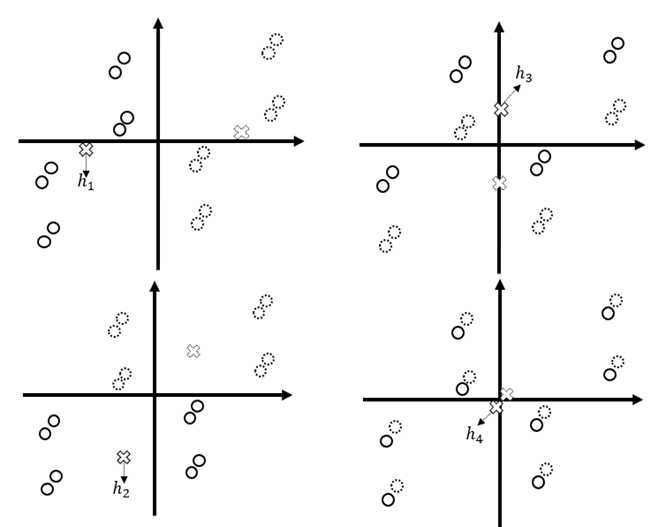
\includegraphics[width=15cm]{fig/structure_check.png}
 \caption{An example of structure check.}
 \label{fig:structure_check}
\end{figure}


\subsubsection{Structure Check}

After the above steps, the estimated superimposed levels can be correctly solved with a very high probability. This step is mainly to detect whether estimated centroids are entirely correct. Because this step requires a higher degree of complexity and will be used in the channel estimation, it is set in the final step detection. 
The fig.\ref{fig:derivation_channel_gain}-(a) is $U = 4$ BPSK transmission where $h_u$ is channel gain $u \in \{ 1,2,3,4 \}$ and the solid circles are the superimposed levels. We can find it has the following characteristics: dividing the superimposed level into two groups: solid circles and dotted circles in fig.\ref{fig:structure_check}. Because of half of the superimposed added with $h_u$ and the other half added with  $-h_u$, we can find the different symmetrical property with $h_u$ ; $u \in \{ 1,2,3,4 \}$ as the center. If it conforms to the structure, we can be very sure that the estimated centroids are correct. This structure will also be used in the next section, so there will be a more detailed discussion on how to implement it in the next section .\ref{section:Derivation of Channel Coefficients}.


\subsection{Derivation of Channel Coefficients}
\label{section:Derivation of Channel Coefficients}

We can classify the received symbols into $2^{mU}$ groups by the clustering techniques introduced in Sec.~\ref{s:clustering}, and the centroids of groups are the estimated superimposed levels. Recall that the fading coefficients are constant across a block of $N_t$ consecutive symbols, and the occurrence probabilities of superimposed levels are equally like in assumption. Using the derivation channel coefficient algorithm as following, we can further estimate the channel coefficients of $U$ users from the resultant centroids. In this section, ideal clustering that the centroids are exactly equal to superimposed levels is assumed to clearly illustrate the procedure. 

Before introducing the derivation of the channel coefficients algorithm, we must know how the superposition levels compose, and here we find the rules for its composition. As shown in the fig.\ref{fig:superimposed_levels_composation}, the levels are superimposed from channel gains $h_1$ to $h_4$ in sequence. The fig-(a) is the signal generated by $h_1$. The amplitude and phase of levels are the same as $h_1$ because of the BPSK transmission. The fig-(b) is the superimposed levels generated by $h_1$ and $h_2$. The superimposed levels are obtained by splitting $\pm$ $h_2$ from fig-(a), so the center of these two splitting groups is $\pm$ $h_2$. Fig-(c) is the superimposed levels generated by $h_1$ $h_2$ and $h_3$. Similarly, $\pm$ $h_3$ can be added to the four levels in fig-(b) separately, so it can be split into eight levels. Then, we can derive $2^{mU}$ superimposed levels from $U$ channel gains, which is the rule of superimposed signals. On the contrary, we can also derive channel gains from superimposed signals by the iterative process.
\\



\begin{figure}[t!]
 \centering
 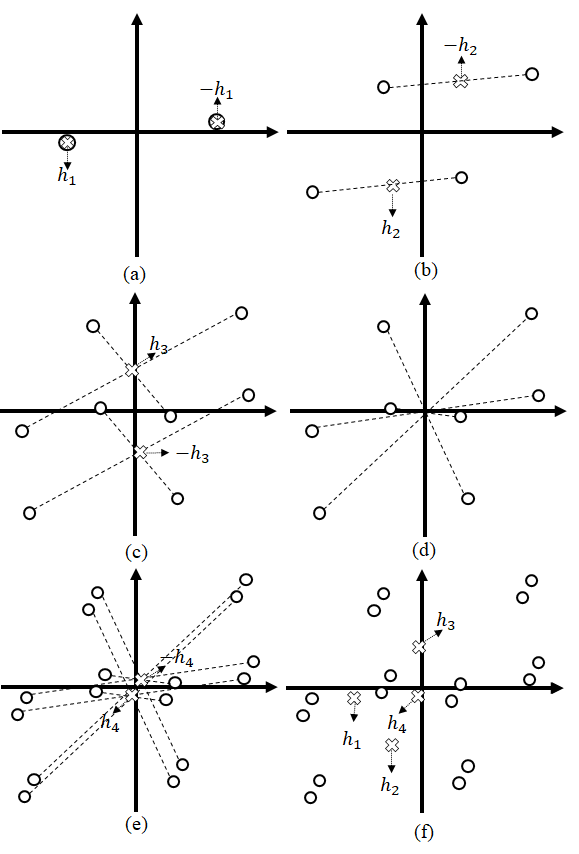
\includegraphics[width=15cm]{fig/superimposed_levels_composation.png}
 \caption{The steps to compose superimposed levels.}
 \label{fig:superimposed_levels_composation}
\end{figure}

From the rule of superimposed level composition,  channel gains can be solved one by one, which removes the level of information of solved gains. In this way, we only need to find the remaining channel gains, which can save a lot of operations. The steps of the derivation of channel coefficients is organized as follows.


\begin{enumerate}[leftmargin=\leftmargin+\widthof{Prefix}]
\item[Step 1)] Pair the $2^{mU}$ levels with the sum of each pair is equal to zero according to modulation.
\item[Step 2)] Group $2^{mU}$ levels into $2m$ groups, each signal of groups are not in the same pair, and derive the centroids of each group, where $m$ is the modulation order.
\item[Step 3)] Return to Step 2 until each group is symmetrical with their centroids.
\item[Step 4)] Derive the channel coefficient that is the group centroid.
\item[Step 5)] Shift $2m$ groups to the original point.
\item[Step 6)] Return to Step 1 and $U=U-1$ until all coefficients are derived.
\end{enumerate}

Fig.\ref{fig:derivation_channel_gain} is process of derivation of channel coefficient. The first step is to pair the centroids with each pair's sum equal to zero in fig-(b).  Step 2 is the brute force method for getting all compositions, and there are $2^{2^{mU}-1}$ combinations in total, but only $2mU$ combinations are correct that is an exponential operation according to $U$ user. Fig-(b) is the false case, and fig-(c) is the correct case. Then, deposit the derived estimated channel gain, which is the centroid of the two groups. We only need to derive the remaining channel gains. According to modulation order $m$, the group number is also different. In step 5, shift the symmetrical groups into the original point and average the pair levels, which can reduce $2^{mU}$ levels into $2^{mU-1}$ levels as fig-(e).


\begin{figure}[t!]
 \centering
 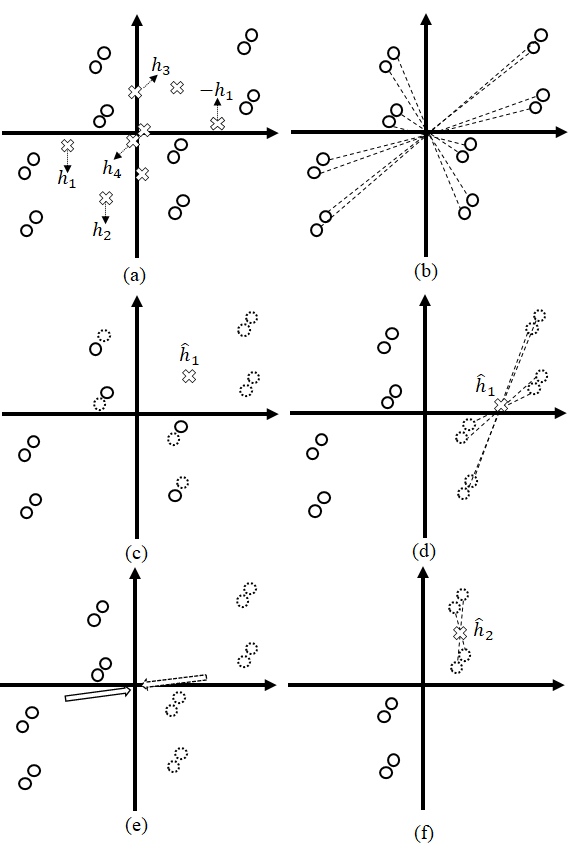
\includegraphics[width=15cm]{fig/derivation_channel_gain.png}
 \caption{The steps of derivation of channel coefficients.}
 \label{fig:derivation_channel_gain}
\end{figure}

The fig.\ref{fig:derivation_channel_gain} is an example of $U=4$, BPSK transmission for deriving channel gains. The first step is to pair all levels. After pairing, group levels into two groups with the restrictions, as shown in (c), it is obvious that the levels in fig-(c) are not symmetrical with their centroids. Therefore, return to step 2 and generate two groups again until it meets the symmetrical condition, as shown in fig-(d). Then, shift the corresponding groups to the original point, and search the remaining levels for deriving rest channel gains.

Compared with the previous geometric method, the novel method does not limit the size of $U$, even if the modulation is different. In terms of implementation, the method only needs a loop to make it work. Compared with the previous implementation complexity, which has been improved a lot. However, in terms of computational complexity, especially in step 2, it will grow exponentially with the $U$ users, which might be improved in future work.

\begin{figure}[t!]
 \centering
 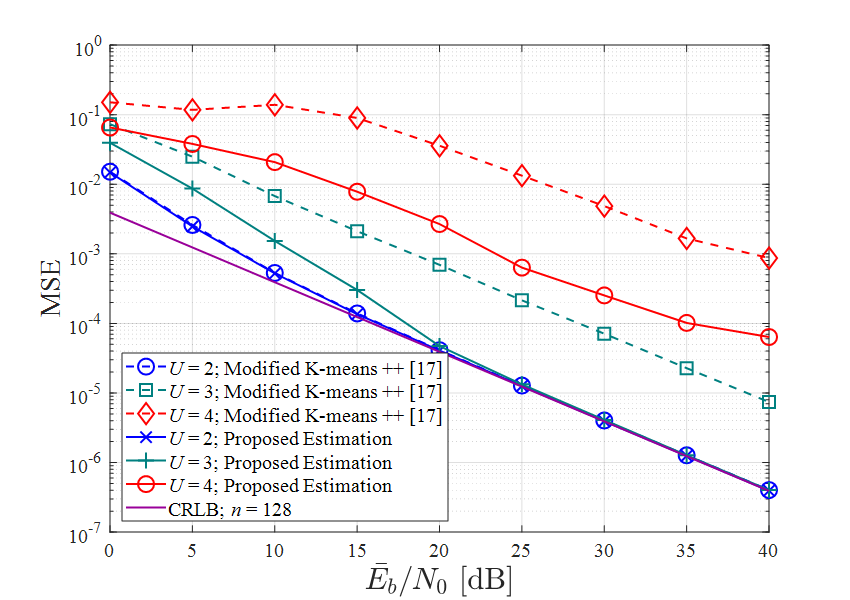
\includegraphics[width=14cm]{fig/channel_gain_mse_128.png}
 \caption{The MSE of estimated channel gain at $N_t=128$. GMM is used.}
 \label{fig:channel_gain_mse_128}
\end{figure}

\begin{figure}[t!]
 \centering
 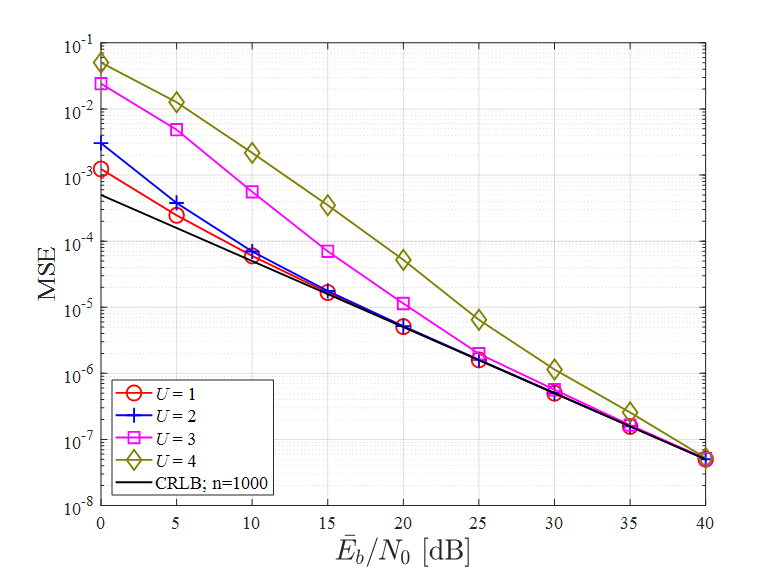
\includegraphics[width=14cm]{fig/channel_gain_mse_1000.png}
 \caption{The MSE of estimated channel gain at $N_t=1000$. GMM is used.}
 \label{fig:channel_gain_mse_100}
\end{figure}


Fig.\ref{fig:channel_gain_mse_128} is the MSE performance of estimated channel gain in a different algorithm, where we compare the navel algorithm with the previous algorithm in \cite{hsu2020uplink}. Assume received samples $N_t=128$. When $U=3$, the proposed algorithm can approach CR bound. Compared with paper \cite{hsu2020uplink}, the effect is excellent, and when $U=4$, it is also good. Because there are too few samples, there is no way to ensure that all superimposed levels are reliable, so it still can not approach CRLB. When the number of samples is increased, we can solve this problem. Fig.\ref{fig:channel_gain_mse_100} is the MSE of $N_t=1000$, When high SNR, $U=4$ can still be close to CRLB. As long as the sample is enough, the proposed clustering algorithm can achieve CRLB.


\section{Resolving Phase Ambiguity}
\label{s:ambiguity}

Although we can have the estimates of channel coefficients through the clustering, there is still an uncertain phase ambiguity due to the estimation using signals that carry messages. An easy way to remove the uncertainty(ambiguity) is to differentially encode the message. However, the differential encoding results in a loss of error performance because of error propagation. Hence, several methods like differential encoder, BCJR decoder, joint decoding, and NBC are introduced to solve phase ambiguity in the thesis \cite{yt19}. Here, we introduce a novel method called $ Q $-section NBC using the polar code structure. In a single carrier system, only need NBC to resolve the phase ambiguity but can not in $Q$ multiple carrier system since there are $Q$ phase ambiguities in a codeword. In this section, we introduce differential encoder, NBC, Q-section NBC in sequence.

\subsection{Differential Encoding}

Differentially encoded (DE) modulation uses the difference between symbols to carry a message. In the transmission of PSK, a message is embedded in the difference of phases between two consecutive symbols, and coherent detection can still be applied, resulting in differentially encoded coherently detected PSK (DE-PSK). Therefore, the phase offset resulted from uncertain ambiguity in blind estimation will not affect the detection of data in DE-PSK transmissions. The block diagram of the DE-BPSK scheme is provided in Fig.~\ref{fig:de_bpsk_enc}.

\begin{figure}[t!]
 \centering
 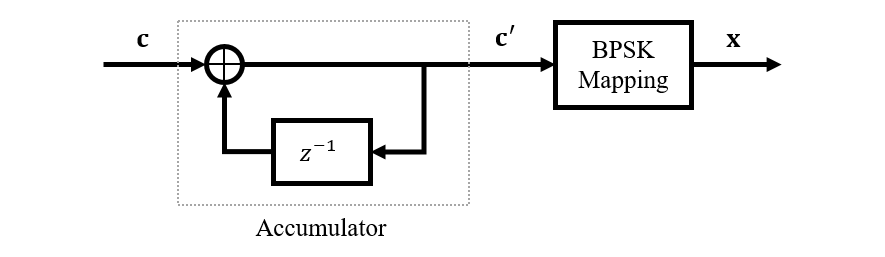
\includegraphics[width=15cm]{fig/de_bpsk_enc.png}
 \caption{Modulation scheme for DE-BPSK transmission.}
 \label{fig:de_bpsk_enc}
\end{figure}

\subsection{Noncoherent Block-Coded Modulation}

In \cite{nbc05}, a novel block-coded modulation (BCM) scheme with noncoherent detection called noncoherent block-coded MPSK (NBC-MPSK) was proposed. The ambiguity can be easily removed without applying differential encoding by partitioning the code space as long as the generator matrix of a linear block code containing an all-one row.

The original code space $C'$ is divided into $C'=\{C, C \oplus \bf 1\}$, where $\bf 1$ is an all-one vector, and the generator matrix $\bf G$ of $C$ is found by removing the all-one row in the generator matrix of $C'$. We only select the codewords from $C$ to be transmitted, i.e., encode the message with $\bf G$, resulting in a rate loss of one bit. At the receiver side, if the signal is BPSK-modulated, the codeword $\bf c'$ corresponding to the received signal would be $\bf c$ or ${\bf c} \oplus {\bf 1}$ due to an uncertain phase ambiguity of $180^{\circ}$ where $\bf c$ is the transmitted codeword in $C$. To remove the uncertain ambiguity, we just need to detect whether the decoded codeword $\tilde{\bf c}$ is in $C$ or not and the resultant codeword is
\begin{equation}
 \hat{\bf c} =
  \begin{dcases}
   \ \tilde{\bf c}, & \text{if } \tilde{\bf c} \in C \\
   \ \tilde{\bf c} \oplus {\bf 1}, & \text{if } \tilde{\bf c} \not\in C
  \end{dcases}
\label{equ:space_identification}
\end{equation}

\begin{figure}[t!]
 \centering
 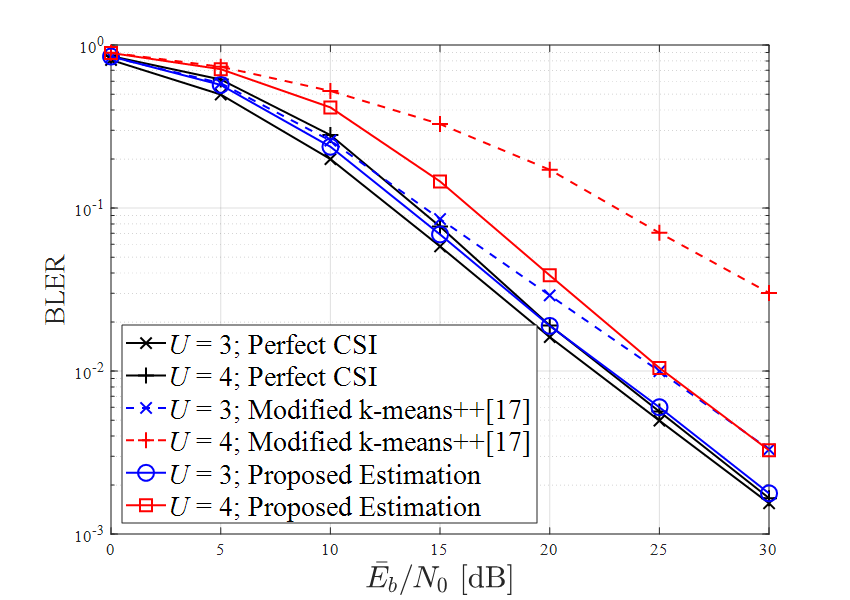
\includegraphics[width=15cm]{fig/bler_polar_channel_estimation.png}
 \caption{BLER performances for a (128,64) Polar-coded GDMA system over
quasi-static Rayleigh flat-fading single carrier channels. NBC and GMM are both used.}
 \label{fig:bler_polar_channel_estimation}
\end{figure}


For a higher-order modulation scheme, the multi-level coding in BCM can be decoded by multi-stage decoding, as shown in \cite{nbc05}. The code space identification in (\ref{equ:space_identification}) can be implemented by checking the number of satisfied parity-check equations. However, the bit errors after decoding might result in erroneous identification and redundant bit-flipping. 

We consider the (128, 64) Polar-coded and the BPSK modulated GDMA system over quasi-static Rayleigh fading channels based on perfect timing. The block error rate (BLER) performances from the simulation are provided in fig. \ref{fig:bler_polar_channel_estimation}. Successive cancellation list (SCL) decoding is used where the list size is 32. Set n = 128. In this case, the phase ambiguity is resolved via NBC. For $U = 3$ and $U = 4$, the BLER using proposed estimation algorithm is obviously better than algorithm in \cite{hsu2020uplink}.

\subsection{Section Noncoherent Block-Coded Modulation}

Consider a codeword transmits into a multi-carrier system and passes through a $Q$ multi-carrier system. Since the cluster-based channel estimation still has the phase ambiguity problem in each sub-carrier channel gains, the received codeword might be split into $Q$ segments. For example, codeword 0000 passes through a two multi-carrier system. The received codeword may be 0011, 1100, 0000, 1111 , and the Q-section NBC was proposed to solve this problem.

In Q-section NBC, the original code space $C'$ is divided into $C'=\{C, C \oplus {\bf{v_1}}, C \oplus {\bf{v_2}}, \cdots, C \oplus {\bf{v_Q}} \}$, where ${\bf{v_i}}, i \in \{ 1, \cdots, Q \}$ are the vectors for splitting the code space, and the generator matrix $\bf G$ of $C$ is found by removing all control vectors in the generator matrix of $C'$. We only select the codewords from $C$ to be transmitted, i.e., encode the message with $\bf G$, which results in a rate loss of $Q$ bit. The control vectors $v_i$ are designed according to multi carrier mapping as following matrix ${\bf V} = {[{\bf{v_1}} \ {\bf{v_2}} \ \cdots \ {\bf{v_Q}}]}^{\text{T}}$.

Assume that the code length $N=2^n$, the section $Q=2^q$, ${\bf{v_0}}$ is an all-one vector. Firstly, generate the control vectors $v_i, i \in \{ 1 \ , 2 , \cdots , q-1 \}$, and the ${\bf{v_i}}$ is described as \ref{equ:v_i}. Then, utensil $j$ control vectors ${\bf{v_i}}$ to generate remaining vectors, where $j \in \{  1, \ , 2 , \cdots , q \}$ is the combination number. Finally, we would derive $Q$ vectors, where $Q=2^q=1+C^q_1+C^q_2+\cdots+C^q_q$.




\begin{align}
{\bf{v_i}} = {( \underbrace{1 \cdots 1}_{2^{n-i}} \ \underbrace{0 \cdots 0}_{2^{n-i}} \ \underbrace{1 \cdots 1}_{2^{n-i}} \ \underbrace{0 \cdots 0}_{2^{n-i}})}; i \in \{ 1, \ 2, \cdots , q  \}.
\label{equ:v_i}
\end{align}

The equation.\ref{equ:section_NBC_1} is an example for $N=8$ and $Q=4$. Generate ${\bf{v_1}}$ and ${\bf{v_2}}$ according to section $q=2$, and derive ${\bf{v_3}}={\bf{v_1}} \oplus {\bf{v_2}}$.  
\begin{equation}
{\bf V}= {
\left[ \begin{array}{ccc}
{\bf{v_0}} \\
{\bf{v_1}} \\
{\bf{v_2}} \\
{\bf{v_3}}
\end{array} 
\right ]}= {
\left[ \begin{array}{ccc} 
\bf v_0 \\
\bf  v_1 \\
\bf  v_2 \\
\bf  v_1 \oplus v_2
\end{array} 
\right ]} 
= {
\left[ \begin{array}{cccccccc}
1 & 1 & 1 & 1 & 1 & 1 & 1 & 1\\
1 & 1 & 1 & 1 & 0 & 0 & 0 & 0\\
1 & 1 & 0 & 0 & 1 & 1 & 0 & 0\\
1 & 1 & 0 & 0 & 0 & 0 & 0 & 0
\end{array}
\right ]}; \ Q=4; \ N=8
\label{equ:section_NBC_1}
\end{equation}


The equation.\ref{equ:section_NBC_2} is an example for $N=16$ and $Q=8$. Generate $\bf v_0, \ v_1, \ v_2, \ v_3$ according to section $q=4$. Then, derive $\bf v_4, v_5, v_6$, which is combined by two vectors and $\bf v_7$ is combined by three vectors. 
\begin{equation}
{\bf V} = {
\left[ \begin{array}{ccc}

\bf v_0 \\
\bf v_1 \\
\bf v_2 \\
\bf v_3 \\
\bf v_1 \oplus v_2 \\
\bf v_1 \oplus v_3 \\
\bf v_2 \oplus v_3 \\
\bf v_1 \oplus v_2 \oplus v_3
\end{array} 
\right ]} = {
\left[ \begin{array}{cccccccccccccccc}
1 & 1 & 1 & 1 & 1 & 1 & 1 & 1 & 1 & 1 & 1 & 1 & 1 & 1 & 1 & 1\\
1 & 1 & 1 & 1 & 1 & 1 & 1 & 1 & 0 & 0 & 0 & 0 & 0 & 0 & 0 & 0\\
1 & 1 & 1 & 1 & 0 & 0 & 0 & 0 & 1 & 1 & 1 & 1 & 0 & 0 & 0 & 0\\
1 & 1 & 0 & 0 & 1 & 1 & 0 & 0 & 1 & 1 & 0 & 0 & 1 & 1 & 0 & 0\\
1 & 1 & 1 & 1 & 0 & 0 & 0 & 0 & 0 & 0 & 0 & 0 & 0 & 0 & 0 & 0\\
1 & 1 & 0 & 0 & 1 & 1 & 0 & 0 & 0 & 0 & 0 & 0 & 0 & 0 & 0 & 0\\
1 & 1 & 0 & 0 & 0 & 0 & 0 & 0 & 1 & 1 & 0 & 0 & 0 & 0 & 0 & 0\\
1 & 1 & 0 & 0 & 0 & 0 & 0 & 0 & 0 & 0 & 0 & 0 & 0 & 0 & 0 & 0
\end{array}
\right ]}; \ Q=8; \ N=16
\label{equ:section_NBC_2}
\end{equation}

Matrix.\ref{equ:section_polar_construction} is the polar code construction for $N=16$. The section NBC control vector $\bf{v_i}$ is the $\frac{N}{Q} \cdot i$-th row of polar code structure, $i = 1 , \cdots, Q$. If $\bf{v_i}$ is information bits for polar code,  we do not put message on it. Since the ambiguity phase shift, these bits are used for control phase, e.g., they are not message bits. If $\bf {v_i}$ is frozen bits for polar code, different from conventional SCL decoding, we can not feedback $0$ for message passing. Since these bits are also used for control phase, it might be $0$ or $1$ randomly. Here, we use list to record these frozen bits for fetching up this issue. \ref{fig:bler_gdma_ofdm_polar_sectionNBC} is the BLER performance for 16 phase ambiguity polar coded OFDM system. where SCD SCL-32 is used.



\begin{equation}
{\begin{array}{ccc}
\\ \bf v_1 \oplus v_2 \oplus v_3 & \longrightarrow \\
\\ \bf v_1 \oplus v_2 & \longrightarrow \\
\\ \bf v_1 \oplus v_3 & \longrightarrow \\
\\ \bf v_1  & \longrightarrow \\
\\ \bf v_2 \oplus v_3 & \longrightarrow \\
\\ \bf v_2 & \longrightarrow \\
\\ \bf v_3 & \longrightarrow \\
\\ \bf v_0 & \longrightarrow \\
\end{array} 
} 
{\left[ \begin{array}{cccccccccccccccc}
1 & 0 & 0 & 0 & 0 & 0 & 0 & 0 & 0 & 0 & 0 & 0 & 0 & 0 & 0 & 0\\
1 & 1 & 0 & 0 & 0 & 0 & 0 & 0 & 0 & 0 & 0 & 0 & 0 & 0 & 0 & 0\\
1 & 0 & 1 & 0 & 0 & 0 & 0 & 0 & 0 & 0 & 0 & 0 & 0 & 0 & 0 & 0\\
1 & 1 & 1 & 1 & 0 & 0 & 0 & 0 & 0 & 0 & 0 & 0 & 0 & 0 & 0 & 0\\
1 & 0 & 0 & 1 & 0 & 0 & 0 & 0 & 0 & 0 & 0 & 0 & 0 & 0 & 0 & 0\\
1 & 1 & 0 & 1 & 1 & 0 & 0 & 0 & 0 & 0 & 0 & 0 & 0 & 0 & 0 & 0\\
1 & 0 & 1 & 0 & 1 & 0 & 0 & 0 & 0 & 0 & 0 & 0 & 0 & 0 & 0 & 0\\
1 & 1 & 1 & 1 & 1 & 1 & 1 & 1 & 0 & 0 & 0 & 0 & 0 & 0 & 0 & 0\\
1 & 0 & 0 & 0 & 0 & 0 & 0 & 0 & 1 & 0 & 0 & 0 & 0 & 0 & 0 & 0\\
1 & 1 & 0 & 0 & 0 & 0 & 0 & 0 & 1 & 1 & 0 & 0 & 0 & 0 & 0 & 0\\
1 & 0 & 1 & 0 & 0 & 0 & 0 & 0 & 1 & 0 & 1 & 0 & 0 & 0 & 0 & 0\\
1 & 1 & 1 & 1 & 0 & 0 & 0 & 0 & 1 & 1 & 1 & 1 & 0 & 0 & 0 & 0\\
1 & 0 & 0 & 0 & 1 & 0 & 0 & 0 & 1 & 0 & 0 & 0 & 1 & 0 & 0 & 0\\
1 & 1 & 0 & 0 & 1 & 1 & 0 & 0 & 1 & 1 & 0 & 0 & 1 & 1 & 0 & 0\\
1 & 0 & 1 & 0 & 1 & 0 & 1 & 0 & 1 & 0 & 1 & 0 & 1 & 0 & 1 & 0\\
1 & 1 & 1 & 1 & 1 & 1 & 1 & 1 & 1 & 1 & 1 & 1 & 1 & 1 & 1 & 1\\
\end{array}
\right ]}
\label{equ:section_polar_construction}
\end{equation}


\begin{figure}[t!]
 \centering
 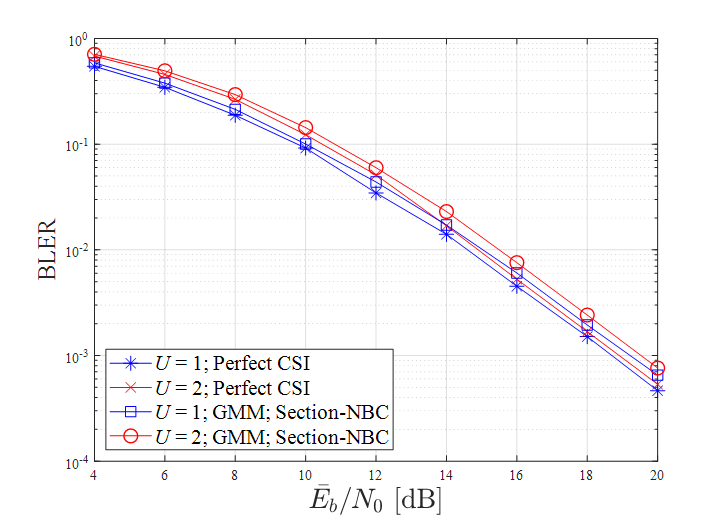
\includegraphics[width=15cm]{fig/bler_gdma_ofdm_polar_sectionNBC.png}
 \caption{BLER performances of Polar-coded GDMA OFDM systems over quasi-static Rayleigh flat-fading channels with 16-subcarrier.}
 \label{fig:bler_gdma_ofdm_polar_sectionNBC}
\end{figure}




